
%%%%%%%%%%%%%%%%%%%%%%%%%%%%%%%%% Preamble %%%%%%%%%%%%%%%%%%%%%%%%%%%%%%%%%%%


\documentclass{beamer}


\usetheme{AnnArbor}


\usepackage{perpage} % makes foonotes per page with a commmand
\usepackage{graphicx}
\usepackage{booktabs}
\usepackage{amsmath}
\usepackage{dcolumn}
\usepackage{caption}
\usepackage{tikz}


\setbeameroption{show notes on second screen} % comment out this line to get without notes version for the purpose of distribution
% \setbeameroption{show notes} % note pages are interleaved with slides
% \setbeameroption{hide notes}
\MakePerPage{footnote} % pkg: perpage, makes footnotes per page
\graphicspath{{./imgs/}} % pkg: graphicx, direcoty of images
\DeclareMathOperator{\E}{\mathbb{E}} % pkg: amsmath
\newcolumntype{d}[1]{D{.}{.}{#1}} % pkg: dcolumn
\setbeamertemplate{caption}[numbered] % make table and figs numbered


\title[Ng, Wu (2007)]{\MakeUppercase{The trading behavior of institutions and individuals in Chinese equity markets}}
\subtitle{Journal of Banking \& Finance (2007)}
\author[Mahdi Mir]{Lilian Ng\texorpdfstring{\footnote{Lubar School of Business, University of Wisconsin-Milwaukee \newline Now: Schulich School of Business, York University}}{}, Fei Wu\texorpdfstring{\footnote{Massey University, Department of Finance, New Zealand \newline Now: Shanghai Advanced Institute of Finance}}{}}
\date[TeIAS]{\today}


%%%%%%%%%%%%%%%%%%%%%%%%%%%%%%%%% Begin Doc %%%%%%%%%%%%%%%%%%%%%%%%%%%%%%%%%%


\begin{document}

\begin{frame}
    \titlepage{}
\end{frame}

\begin{frame}[label=outl]
    \frametitle{Outline}
    \tableofcontents{}
\end{frame}


\section{Introduction}

\begin{frame}
    \frametitle{Why It is Important?}
    \begin{itemize}
        \item The Chinese equity markets are dominated by individuals.
              \begin{itemize}
                  \item Compared to developed equity markets where a form of polarization between individual and institutional investors is evident.
                  \item 99.5\% individuals, just 0.5\% are institutional. \\ (Chinese Securities Depository \& Clearing Co. Ltd, 2002).
              \end{itemize}
        \item Chinese markets were only established in the early 90s.
        \item Short-selling \& margin trading are not allowed in China, like in Iran.
    \end{itemize}
    \begin{tikzpicture}[remember picture, overlay]
        \node[shift={(0em,4em)}]() at (current page.south)
        {
            \hyperlink{outl}{\beamerbutton{Outline}}
        };
    \end{tikzpicture}
\end{frame}


\section{Data}


\subsection*{The Main Data}


\begin{frame}
    \frametitle{The Main Data}
    \begin{itemize}
        \item A Sample of trade-level data executed on the SHSE\footnote{The Shanghai Stock Exchange}
              \begin{itemize}
                  \item Time frame: April 2001-August 2002
                  \item Similar in-sample distribution of individual and institutional accounts to those of the whole market
                  \item The final sub-sample used consists of \(4.72M\) individual and \(11.6K\) institutional accounts.
              \end{itemize}
              \begin{figure}[b]
                  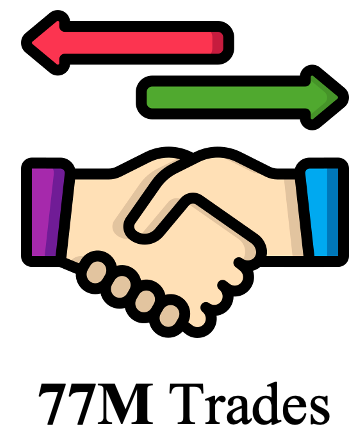
\includegraphics[width= .15\textwidth]{trade1.png}
                  \hspace{2em}
                  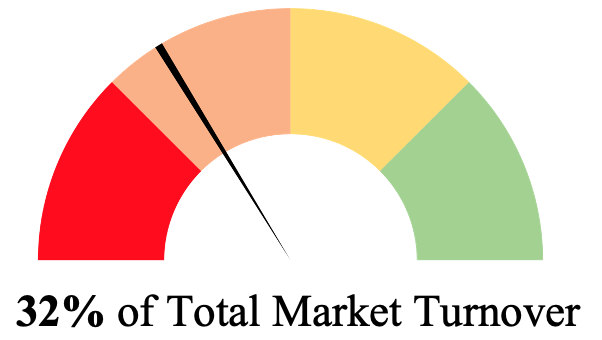
\includegraphics[width= .3\textwidth]{turnover.png}
                  \hspace{2em}
                  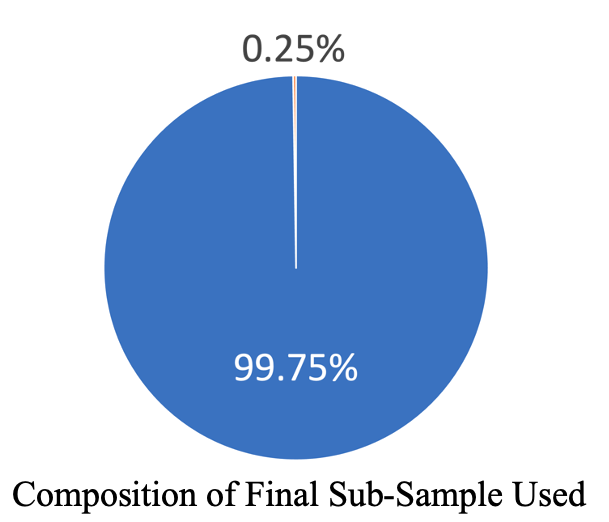
\includegraphics[width= .3\textwidth]{composition.png}
              \end{figure}
    \end{itemize}
\end{frame}


\subsection*{Sample Description}


\begin{frame}
    \begin{table}
        \caption{Aggregate Statistics for Each Group}
        {\fontsize{9}{12} \selectfont
            \begin{tabular}{l*{4}{c}}
                \toprule
                                    & Institutional & \multicolumn{3}{c}{Individual Investors Grouped by Trade Value}                            \\
                \cmidrule(r){3-5}
                                    &               & Largest                                                         & Middle Group & Smallest  \\

                \midrule

                No.\ of Accounts    & 11,586        & 319,675                                                         & 1,767,112    & 2,636,871 \\
                                    & (0.24\%)      & (6.75\%)                                                        & (37.32\%)    & (55.69\%) \\
                \addlinespace

                No.\ of Trades (M)  & 0.24          & 5.12                                                            & 29.73        & 38.84     \\
                                    & (0.33\%)      & (6.93\%)                                                        & (40.21\%)    & (52.53\%) \\
                \addlinespace

                Value of Trades (B) & 98.12         & 687.08                                                          & 584.46       & 223.54    \\
                                    & (6.16\%)      & (43.13\%)                                                       & (36.68\%)    & (14.04\%) \\
                \bottomrule
            \end{tabular}
        }
    \end{table}
\end{frame}

\begin{frame}
    \begin{table}
        \caption{Statistics by Type of Trading Activity}
        {\fontsize{6}{12} \selectfont
            \begin{tabular}{l*{8}{d{2}}}
                \toprule
                                          &                                   &                             & \multicolumn{6}{c}{Individual investors grouped by trade value}                                                                                                                                          \\
                \cmidrule(r){4-9}
                                          & \multicolumn{2}{c}{Institutional} & \multicolumn{2}{c}{Largest} & \multicolumn{2}{c}{Middle group}                                & \multicolumn{2}{c}{Smallest}                                                                                                           \\
                \cmidrule(r){2-3} \cmidrule(r){4-9}
                                          & \multicolumn{1}{c}{Buy}           & \multicolumn{1}{c}{Sell}    & \multicolumn{1}{c}{Buy}                                         & \multicolumn{1}{c}{Sell}     & \multicolumn{1}{c}{Buy} & \multicolumn{1}{c}{Sell} & \multicolumn{1}{c}{Buy} & \multicolumn{1}{c}{Sell} \\
                \midrule

                No.\ of Trades (M)        & 0.12                              & 0.12                        & 2.61                                                            & 2.51                         & 15.65                   & 14.07                    & 20.57                   & 18.27                    \\
                \addlinespace

                No.\ of Shares Traded (B) & 14.03                             & 12.8                        & 43.18                                                           & 42.77                        & 32.47                   & 31.47                    & 12.95                   & 12.22                    \\
                \addlinespace

                Trade Value (B)           & 51.99                             & 46.13                       & 348.37                                                          & 338.72                       & 298.44                  & 286.02                   & 115.52                  & 108.03                   \\
                \bottomrule
            \end{tabular}
        }
    \end{table}
    \begin{tikzpicture}[remember picture, overlay]
        \node[shift={(0em,4em)}]() at (current page.south)
        {
            \hyperlink{outl}{\beamerbutton{Outline}}
        };
    \end{tikzpicture}
\end{frame}


\section{Investor Groups' Trading Pattern}


\subsection*{Measures}


\begin{frame}
    \frametitle{Investor Groups' Trading Pattern}
    \framesubtitle{Measures of Excess Buying (Selling)}
    \begin{itemize}
        \item A measure of net buying (selling) of stock \(i\) by investor group \(G\). \(g = 1,\ldots,N_G\) is an investor in group \(G\).
              \[
                  \mathrm{NB}_{i, t}^{G} = \frac{\sum_{g=1}^{N_{G}} \mathrm{Buy}_{i, t}^{g}-\sum_{g=1}^{N_{G}} \mathrm{Sell}_{i, t}^{g}}{\sum_{g=1}^{N_{G}} \mathrm{Buy}_{i, t}^{g}+\sum_{g=1}^{g} \mathrm{Sell}_{i, t}^{g}} = - \mathrm{NS}_{i, t}^{G}
              \]
        \item \(\E(\mathrm{B}_{i,t}^G)=\frac{\sum_{i=1}^{N_{t}^{G}} \mathrm{NB}_{i, t}^{G}}{N_{t}^{G}} = - \E(\mathrm{S}_{i,t}^G)\)
        \item By adjusting for the group's average excess buying and selling of all stocks at time \(t\), define two measures for excess buying and selling of each stock by investor group \(G\).
              \[
                  \mathrm{XB}_{i, t}^{G} = \mathrm{NB}_{i, t}^{G} - \E(\mathrm{B}_{i,t}^G) = - \mathrm{XS}_{i, t}^{G}
              \]
    \end{itemize}
\end{frame}


\subsection*{Variables}


\begin{frame}
    \frametitle{Independet and Control Variables}
    \begin{itemize}
        \item Returns prior to trading day are independent variables.
        \item Dummies for contemporaneous and one-day lagged stock-specific ``good'' and ``bad'' news
        \item Dummies for capturing day-of-the-week effect
        \item A dummy for IPO
        \item Two dummies for ``reference point'' effects
    \end{itemize}
\end{frame}


\subsection*{Results}


\begin{frame}
    \begin{table}
        \caption{\label{tab:res}Investor Trading Decisions and Past Stock Returns}
        {\fontsize{6}{11} \selectfont
            \begin{tabular}{l*{8}{c}}
                \toprule
                                & \multicolumn{2}{c}{Institutional} & \multicolumn{6}{c}{Individual Investors Grouped by Trade Value}                                                                                                                                \\
                \cmidrule(r){4-9}
                                &                                   &                                                                 & \multicolumn{2}{c}{Largest} & \multicolumn{2}{c}{Middle group} & \multicolumn{2}{c}{Smallest}                                \\
                \cmidrule(r){2-3} \cmidrule(r){4-9}
                                & Buy                               & Sell                                                            & Buy                         & Sell                             & Buy                          & Sell    & Buy      & Sell    \\
                \midrule
                \(R(-1)\)       & 0.690**                           & -0.384                                                          & 0.941**                     & -0.481**                         & -0.430**                     & 1.477** & -2.725** & 2.882** \\
                                & (2.22)                            & (-0.98)                                                         & (8.54)                      & (-4.08)                          & (-6.88)                      & (22.3)  & (-39.2)  & (38.8)  \\
                \addlinespace

                \(R(-2,-5)\)    & 0.188                             & -0.494**                                                        & 0.137**                     & 0.088*                           & -0.503**                     & 0.710** & -0.967** & 0.821** \\ % chktex 8
                                & (1.26)                            & (-2.72)                                                         & (2.67)                      & (1.71)                           & (-17.2)                      & (24.6)  & (-29.8)  & (25.4)  \\
                \addlinespace
                \(R(-6,-27)\)   & 0.080                             & -0.170*                                                         & -0.034                      & 0.098**                          & -0.189**                     & 0.251** & -0.322** & 0.263** \\
                                & (1.01)                            & (-1.91)                                                         & (-1.31)                     & (3.86)                           & (-12.7)                      & (17.5)  & (-19.4)  & (16.4)  \\
                \addlinespace
                \(R(-28,-119)\) & -0.068                            & 0.067                                                           & -0.043**                    & 0.024                            & -0.089**                     & 0.107** & -0.094** & 0.121** \\
                                & (-1.17)                           & (1.14)                                                          & (-2.67)                     & (1.41)                           & (-9.71)                      & (11.2)  & (-9.22)  & (11.3)  \\
                \addlinespace

                \(R^{2}\)       & 0.07\%                            & 0.08\%                                                          & 0.31\%                      & 0.28\%                           & 0.63\%                       & 1.14\%  & 3.30\%   & 3.14\%  \\
                Obs             & 50004                             & 50004                                                           & 175527                      & 175527                           & 182115                       & 182115  & 181755   & 181755  \\

                \bottomrule

                \addlinespace[1ex]

                \multicolumn{2}{l}{\textsuperscript{**}\(p<0.05\), \textsuperscript{*}\(p<0.1\)}
            \end{tabular}
        }
    \end{table}

    \begin{tikzpicture}[remember picture, overlay]
        \node[shift={(0em,2em)}]() at (current page.south)
        {
            \hyperlink{outl}{\beamerbutton{Outline}}
        };
    \end{tikzpicture}


    \note<1>[item]{The model employs the panel data fixed effects OLS\@.}
    \note<1>[item]{The dependent variables are excess buys and excess sells of each investor group, as defined earlier.}
    \note<1>[item]{The independent variables are past positive (negative) stock performance over varying time intervals and all stock-specific controls.}

    \note<2>[item]{Table\ \ref{tab:res}  shows systematic and consistent patterns of past-returns effects on the trading activities of different groups of investors.}
    \note<2>[item]{Ins act as momentum traders in both buy and sell}
    \note<2>[item]{
        Coefficient on R (-1) is 0.69 with PCSE-adjusted t-statistic of 2.2.
        \begin{itemize}
            \item whereas their counterpart return coefficients of longer horizons are all statistically insignificant.
        \end{itemize}
    }
    \note<2>[item]{Ins sell more poorly performing stocks.
        \begin{itemize}
            \item Coefficients on R (-2,-5) and R (-6,-27) are -0.49 and -0.17 and at least at the 10\% level.
        \end{itemize}
    }
    \note<3>[item]{Like insts, the wealthiest individuals also pursue momentum investing, especially in the buys than sells.
        \begin{itemize}
            \item The buy coefficients on both R (-1) and R (-2,-5) for this group of investors are positive and highly significant.
        \end{itemize}
    }
    \note<3>[item]{Wealthiest individuals act more like contrarians when past stock performance is poor.
        \begin{itemize}
            \item their sell coefficients on R (-2,-5) and R (-6,-27) are positive and statistically significant at the 10\% level.
        \end{itemize}
    }
    \note<3>[item]{Finally, the majority of individual investors, who consist of about 93\% of the investing population, are largely contrarians
        \begin{itemize}
            \item Their buy coefficients are all negative and sell coefficients are all positive, and both buy and sell coefficients are statistically significant at conventional levels.
        \end{itemize}
    }
\end{frame}


\section{Impact of Trading on Future Volatility}


\subsection*{Research Design}


\begin{frame}
    \frametitle{Impact of Trading on Future Volatility}
    \framesubtitle{The Model}
    \begin{align*}
        \sigma_{i, t}  = & \phi_{i, 0}+\phi_{1} \operatorname{Max}\left[\mathbf{N B}_{i, t-1}^{G}, 0\right]+\phi_{2} \operatorname{Max}\left[\mathbf{N S}_{i, t-1}^{G}, 0\right]+\phi_{3} \sigma_{i, t-1} \\
                         & +\phi_{4} \sigma_{\mathrm{M}, t}+\phi_{5} r_{i, t-1}+\epsilon_{i, t}
    \end{align*}
    \begin{itemize}
        \item \(\sigma_{i, t}\) is the monthly return volatility of stock \(i\) in month \(t\).
        \item This separates effects of net buying and net selling on future stock volatility, while controlling for the market wide volatility and the stock's own lagged volatility.
    \end{itemize}
    \note<1>[item]{It is important to stress that in estimating (3), we only employ sample of stocks that we can determine both net sellers and net buyers within the sample.
        \begin{itemize}
            \item In other words, for every stock, we identify a group (s) of investors who are net buyers of the stock and a group (s) of investors who are the net sellers that act on the opposite side of the transactions.
            \item This approach allows us to gauge the relative impact of one group's net selling to another's net buying of a stock.
        \end{itemize}
    }
\end{frame}


\subsection*{Results}


\begin{frame}
    \frametitle{Results}
    \begin{itemize}
        \item Only the \textbf{net buying} of stocks by \textbf{wealthiest} individuals and \textit{net selling} by \textit{institutions} help decrease future stock volatility.
              \begin{itemize}
                  \item This observation perhaps suggests that institutions are net sellers of some stocks where the group of wealthiest individual investors are net buyers.
              \end{itemize}
        \item Less wealthy individual investors who are generally small players in the markets exert no influence on the volatility of the stocks.
    \end{itemize}
    \begin{tikzpicture}[remember picture, overlay]
        \node[shift={(0em,4em)}]() at (current page.south)
        {
            \hyperlink{outl}{\beamerbutton{Outline}}
        };
    \end{tikzpicture}
\end{frame}


\section{Impact of Trading on Future Returns}


\subsection*{Research Design}


\begin{frame}
    \frametitle{Impact of Trading on Future Returns}
    \framesubtitle{The Model}
    \begin{align*}
        r_{i, t} = & \delta_{i, 0}+\delta_{1} \operatorname{Max}\left[\mathbf{N B}_{i, t-1}^{G}, 0\right]+\delta_{2} \operatorname{Max}\left[\mathbf{NS}_{i, t-1}^{G}, 0\right]+\delta_{3} r_{\mathrm{M}, t} \\
                   & +\delta_{4} r_{i, t-1}+\eta_{i, t}
    \end{align*}
    \begin{itemize}
        \item If individuals are noise traders, there should be no systematic relation between their trading activity and future stock returns.
        \item In other words, the estimated \(\delta_{1}\) and \(\delta_{1}\) coefficients should be insignificantly different from zero or should bear signs suggesting that future returns are in counter direction to the trading activity.
    \end{itemize}
\end{frame}


\subsection*{Results}


\begin{frame}
    \frametitle{Results}
    \begin{itemize}
        \item Both Chinese institutions and the majority of Chinese individual investors have no predictive power for future stock returns.
              \begin{itemize}
                  \item The evidence that trading by institutions provides no prediction of future stock returns is somewhat surprising.
                  \item This finding contradicts existing evidence that institutions are typically more sophisticated and more informed than individual investors.
                        \note<1>[item]{
                            \begin{itemize}
                                \item It is likely that the trading activities of our sample of institutions do not necessarily reflect the trading behavior of a typically well informed institution.
                                \item Alternatively, it might suggest that it is harder to form any reliable prediction of future stock returns, given the existence of non-fundamental components of Chinese stock prices. A recent study by Mei et al. (2005) finds evidence that speculative trading is an important determinant of Chinese stock prices.
                            \end{itemize}
                        }
              \end{itemize}
        \item To sum, there seems no evidence that the majority of Chinese individual investors are making sound investment decisions.
    \end{itemize}
    \begin{tikzpicture}[remember picture, overlay]
        \node[shift={(0em,4em)}]() at (current page.south)
        {
            \hyperlink{outl}{\beamerbutton{Outline}}
        };
    \end{tikzpicture}
\end{frame}


\section{Summary}


\begin{frame}
    \frametitle{Summary}
    \begin{itemize}
        \item This papers employ a new unique data set at trade-level.
        \item Institutions pursue momentum investing.
        \item Less wealthy groups of individual investors mainly adopt contrarian strategies.
        \item Wealthier Chinese individuals are likely to increase purchases of winner stocks and to decrease sales of loser stocks.
        \item Only the trading activities of institutions and wealthiest individuals can affect future stock volatility.
        \item Chinese investors at large have no predictive power for future stock returns.
    \end{itemize}
\end{frame}
























\end{document}

%%%%%%%%%%%%%%%%%%%%%%%%%%%%%%%%% End Doc %%%%%%%%%%%%%%%%%%%%%%%%%%%%%%%%%%%%
